\chapter{Introduction}\label{chap:intro}

\emph{“Some witty quote about \kl{C}.”}
\vspace{-1.5em}
\begin{flushright}
  \sidecite[][citing someone]{Placeholder}
\end{flushright}

\margintoc[4em]

\paragraph{Thesis Statement}%
Building a verification tool for C is
two parts engineering, and one part theory. The theory is not particularly
sophisticated, but its application at scale present new challenges and
insights.

\begin{enumerate}
    \item Formalisation, heap factoring, and Ott engineering
    \item Memory object model
    \item Tree Carver, buddy allocator update, working with Galois.
\end{enumerate}

\section{C and Verification}

\subsection{The C Programming Language}

Setting the stage: why C, where is it used (Linux kernel).

\subsection{Verification with Separation Logic}

\section{CN:\ C, No bugs!}


\emph{Lots} of examples of CN,\sidenote{`CN' does not stand for anything; its
name is a historical accident.} to introduce each feature (especially ones
discussed later).\sidetextcite{Placeholder}

\begin{marginfigure}
  \ContinuedFloat*
  \begin{mathpar}
      \inferdef{Var}{\vdash{} \Gamma{} \\ (x: A) \in{} \Gamma{}}{\Gamma{} \vdash{} x \ty{} A}\label{rule:cic-var}
  \end{mathpar}
  \caption{Integrate Ott into this system.}\label{fig:cic-var}
\end{marginfigure}

Reference the rule: \ruleref{rule:cic-var} opposite.

\begin{marginfigure}
\ContinuedFloat{}
  \begin{mathpar}
      \inferrule{\Gamma{} \vdash{} A \ty{} \uni{} \\ \Gamma, x: A \vdash{} t \ty{} T}
      {\Gamma{} \vdash{} \l x: A.\ t \ty{} A \to{} T}
    \and
    \inferrule{\Gamma{} \vdash{} f \ty{} A \to{} T \\ \Gamma{} \vdash{} u \ty{} A }{\Gamma{} \vdash{} f\ u \ty{} T}
  \end{mathpar}
  \caption{Ott in here too.}\label{fig:cic-nondep-fun}
\end{marginfigure}

You can see more at work in \cref{fig:cic-nondep-fun}.


\begin{comment}

\emph{“\kl{Coq} is an old man now, and it has a lot of scars.”}
\vspace{-1.5em}
\begin{flushright}
  \sidecite[][citing Assia Mahboubi]{QuantaPA}
\end{flushright}

\margintoc[4em]

This thesis belongs to the domain of \kl[dependent type]{type theory},%
\sidenote{If you do not know what this or any other word in this introduction
means, read on! They will be explained in due time.}
itself at the crossroads between computer science and mathematical logic.
One of the field’s goals is to give theoretical and practical foundations
for software tools helping humans in constructing and verifying proofs –
in the mathematical sense.
Such tools are called \kl{proof assistants}, and \kl{Coq}, the one
on which my work was mainly focused, is central in this thesis.

Over their more than 50 years of existence, proof assistants have
turned into an established technology. This history is both a blessing and a curse: as
the field matured, the tools have become more and more complex, making them more and more
powerful, but also more and more prone to critical bugs hiding in dark corners. At a time
when they are gaining traction in an increasing number of communities
concerned with high trust levels, this simply cannot be.
The historical solution of keeping a small, trusted \kl{kernel}
– the so-called De Bruijn criterion –
is not enough if we wish to keep moving on and integrate new, powerful features
to keep up with the needs of users.

There is a straightforward solution to this:
proof assistants have been used for decades to certify programs correctness.
Why could they not prove \emph{themselves} correct? After all, if this is
the gold standard we demand for software, it should apply first and foremost to the ones
used to justify that trust. For the proof assistant \kl{Coq},
this is the ambition of the \kl{MetaCoq} project,
which aims at providing a drop-in replacement for \kl{Coq}’s \kl{kernel} that has been
proven correct,
even though it handles all the subtleties and quirks of said \kl{kernel}.
No more trusting a complex and ever-evolving implementation, trust the formally validated
\emph{proofs} instead!

But before we can hope to achieve that goal, we need a deeper study of the structures at work
in the \kl{kernel}. In particular, its typing algorithm is \emph{bidirectional}, meaning that
it constantly alternates between the two problems of type \emph{inference} –
finding a type for a term – and type \emph{checking} –
verifying that a type is adequate for a term. While this
structure is crucial in relating the specification of the type system to its implementation,
it has been rather little studied in the context of the
\kl{Calculus of Inductive Constructions} (\kl{CIC}),
the theoretical foundation of \kl{Coq} – but also of the closely related
\kl{Lean}, \kl{Agda}…

This thesis aims at filling that gap, by providing a thorough study of bidirectional \kl{CIC},
formalized in the framework offered by \kl{MetaCoq} project. This is a key
ingredient in the first formal proof of soundness and completeness of a type-checking
algorithm for a realistic proof assistant kernel.
It was also able to uncover bugs in \kl{Coq}’s kernel that had gone unnoticed until then.

But bidirectional typing is also an interesting theoretical tool in its own right,
giving a valuable form of control over computation.
In particular, it is a necessary piece in the design of a gradual extension of
\kl{CIC}, \kl{GCIC}.
\kl{Gradual typing} aims at bringing to programmers both the flexibility of
development offered by dynamic typing, and the strong guarantees given
by static typing, in one and the same system. \kl{GCIC} intends
to bring that flexibility to dependently-typed programming,
and, by using the power of the \kl{Curry-Howard correspondence}, to proof writing.
But this endeavour comes with subtle difficulties,
that can only be solved in a bidirectional setting.

To replace this work in its larger context, this introduction begins with a very
short history of mathematical logic (\cref{sec:logic-history}), which exposes the
main questions of that field. Follows a presentation of the links between logic and
computer science, through \kl{proof assistants} (\cref{sec:proof-assistants}).
Next, \cref{sec:intro-coq-en} focuses more closely on presenting
the research questions I worked on: bidirectional typing, \kl{MetaCoq} and gradual typing.
Finally, \cref{sec:this-thesis} summarizes my contributions to these questions.

\section{A Very Short History of Logic}
\label{sec:logic-history}

\subsection{Syllogisms}

The main question that logic seeks to answer is that of finding criteria in order to determine
if a reasoning is valid. In Western tradition, this challenge can be traced back to the
Antiquity, and particularly to Aristotle's \textit{Organon}.
The main contribution of this work is to introduce the notion of syllogism.
These are simple fragments of reasoning, whose validity stems from the
fixed structure they follow, rather than a specific content.%
\sidenote{The most well-known is probably the \textit{Barbara} syllogism, and example
of which is: \emph{all humans are mortals; Socrates is human; so Socrates is mortal.}}
If complex reasoning is built from assembling such syllogisms, it must necessarily be valid as
a whole, since every assembled fragment is. There are two important ideas at work here.

The first is that reasoning can be valid or not, depending only on its structure,
independently of its content.
It can be syllogisms, but many other systems. We will come across a certain number of them
in this thesis!

The second idea is that of a construction from elementary components.
Starting from a set of rules
we have identified as valid \textit{a priori}, we have a means to ensure the validity
of potentially very complex reasoning: it suffices to check that these
can be decomposed into the base components.

For the Greek philosophers, logic was also conceived as a means towards communication.
The aim was to check one’s own reasoning, but also to be able to convey
it, by fixing a logical formal system.%
\sidenote{Structural rules reasoning should obey, as those of syllogisms.}
A person wanting their conclusion to be accepted by others would only have to express their
reasoning in a perfectly precise way in the framework of such a formal system.

From that point on, the main focus of logic as a discipline
concentrates on this structure which underlies reasoning.
The main challenge is to construct a formal system, adapted to a specific
field of reasoning. In the case we are interested in, mathematical logic, this
allows us to give a precise meaning to what constitutes a valid mathematical proof.


\subsection{The beginning of mathematical logic: towards a formal foundation}[Towards a formal foundation]

Following Aristotle, mathematicians seized logic in order to build a formal system
able to serve as a rigorous foundation for mathematics.
The links between logic and mathematics go back to Greek Antiquity, but
mathematical logic as a standalone discipline really established itself
during the 19\textsuperscript{th} century, thanks to important progress on two main aspects.

The first consisted in freeing mathematical logic from natural languages%
\sidenote{By opposition with the formal languages which appear in mathematics,
  computer science, etc.},
unsuited to a formal description of reasoning, and to instead design a new specific
form of language that could serve as a basis for mathematical reasoning.
An important step here was \citeauthor{Begriffsschrift}'s
\citetitle{Begriffsschrift}~\sidecite{Begriffsschrift}, which, for the first time,
gave a formal language rich enough to express mathematics satisfyingly. Its
major addition was the notion of quantifier, essential to the mathematical vernacular,
as they give a faithful way to account for universal%
\sidenote{For instance: “Every even natural number is the sum of two prime numbers”.}
and existential%
\sidenote{For instance: “There exists a real whose square is 2”.}
properties.

The second aimed at showing that mathematics as a whole could be reconstructed from a
few simple properties. An important step was the reduction of analysis to the properties
of real numbers, followed by constructions of those from arithmetic given almost
simultaneously by – among others – \sidetextcite{Dedekind1872} and
\sidetextcite{Cantor1872} in 1872.
Meanwhile, \sidetextcite{Peano1889} proposed an axiomatization of natural numbers close to the
one still used today. Finally, Cantor again proposed set theory \sidecite{Cantor1883}
as a formalism expressive enough to describe all mathematical object as sets of elements.

\subsection{The foundational crisis of mathematics}[The foundational crisis]

Unfortunately, the system proposed in the \citetitle{Begriffsschrift} is inconsistent!
That is, it is possible to use it to prove falsity, 
making the logical system collapse.%
\sidenote{In a system where falsity is provable, all propositions are,
  which is known as the principle of explosion.
  Such a system, where everything – and its negation – is provable can obviously not
  serve as an adequate foundation for mathematics.
}
This result, due to Russell%
\sidenote{%
  In a letter to Frege in 1902 the latter made made public
  in \textcite[Nachwort p.~253]{Frege1903}.}%
\margincite{Frege1903}
marked the opening of a crisis period.
Indeed, it cast doubt upon the systems that had started to establish
themselves as good candidates to serve as foundations – that of Frege, but
mainly those of Cantor, which were affected by the same difficulties.

A possible solution has been suggested ten years later  by \citeauthor{Whitehead1913} in their
\citetitle{Whitehead1913} \sidecite{Whitehead1913}. This colossal piece of work
not only proposed a formal system avoiding the inconsistency
of \citetitle{Begriffsschrift}. It also built a significant amount
of mathematics in this system, including a construction of integers,
some arithmetic, and finally real numbers.

In parallel, in the continuity of Cantor’s work, \sidetextcite{Zermelo1908} and others
worked towards giving a version of Cantor’s set theory that is consistent. This lead to what
is colloquially referred to as Zermelo-Fraenkel set theory – ZF, or ZFC when the
axiom of choice%
\sidenote{An axiom very useful in numerous branches of mathematics, but which is often treated
separately, as it is both less crucial than the other axioms of ZF and at the root of
counter-intuitive results.}
\sidecite{Zermelo1904} is added –, which also seemed able to serve as a
solid foundation for mathematics.

\subsection{Incompleteness}

The search for a formal system adequate as a foundation for mathematics however hit a
second major difficulty: Gödel’s incompleteness theorem \sidecite{Goedel1931}. It asserts
that a formal system in which one can construct integers such as those of Peano – and so
\textit{a fortiori} any system rich enough to serve mathematician’s needs – cannot
prove its own consistency.%
\sidenote{Unless the system is inconsistent, in which case it can prove \emph{everything},
by virtue on the explosion principle, including its own consistency… and inconsistency!}
Thus, no formal system can serve as a basis for mathematics
with a formal certitude as to its adequacy.
Indeed, as we cannot prove the consistency of the system in itself, it could very well
turn out to be inconsistent, ruining all the efforts put into its use – just like what
happened with Frege’s \citetitle{Begriffsschrift}. And if we were to use a second system
to prove the first consistent, we would only shift the prolem: now we rely on the
consistency of the second system.

A consequence of this theorem is that a system rich enough to found mathematics is
necessarily incomplete.%
\sidenote{%
  This means that there exist independent statements, that is assertions which
  cannot be proven, and whose negation cannot be proven either.
  The consistency of the system under consideration is one example of such a statement.
}
Thus, in what follows, I will never refer to truth in an absolute sense – which could
only be meaningful in a complete system where every statement is true or false –, but
only about provability \emph{relatively to a given system}.

\subsection{A satisfactory situation?}

Despite the difficulties put into light in the beginning of the 20\textsuperscript{th}
century, the research in mathematical logic reached a somewhat satisfactory situation
a few decades later.
First, ZFC is a reasonable formal system on which mathematics can be founded. Moreover,
the mathematical community is overall convinced it would be \emph{theoretically} possible
to write down all mathematics using ZFC\@. This is enough for most of its members,
even if those who attempt to actually give it a try, in the vein of the
\citetitle{Whitehead1913}, are quite few.

In \emph{practice}, however, things are very different. The human development and
verification of formalized mathematics%
\sidenote{%
  That is, effectively expressed in a fixed formal system.}
seems both impossible, and unnecessary.
On the one hand, it would demand a considerable effort, because such mathematics would
require an extremely high level of precision, both from the author of the formal proof
and from the reader. At the same time, this would not significantly reduce the risk of
errors. It would indeed be very hard for humans to check that some reasoning doubtlessly
follows the rules of the system: a tiny error can easily creep inside thousands of pages
of formal reasoning. Finally, describing mathematics in this way would drown the vital
mathematical intuitions, making communication sterile.

If we wish to make formal mathematics practicable, and benefit from the guarantees
they bring while eliminating these crippling defaults, we thus need new tools.

\section{Computers Enter the Scene}
\label{sec:proof-assistants}

A new element however radically modifies the previous situation: the advent of computers.
Indeed, computer science provides new tools, making formalized mathematics both possible
and attracting.

\subsection{Proof assistants}

Computers excel where humans are weak: their speciality is to treat large volumes of
information in a very precise way, exactly the kind of needs brought up when manipulating
formalized mathematics. Therefore, already at the beginning of the 70s,%
\sidenote{With systems like Automath \cite{DeBruijn1970}, or Mizar
  \cite{Rudnicki1992}.}%
\margincite{DeBruijn1970}%
\margincite{Rudnicki1992}
software tools, collectively called \intro{proof assistants}, start to
appear, that are dedicated to writing and verifying formal proofs.
Through the formalization of proofs and the verification by computers that they
actually follow the rules of the underlying logical system, proof assistants open the
door to a level of trust much higher than that allowed by “informal” proofs.
Renowned mathematicians, such as \sidetextcite{Voevodsky2010},
\sidetextcite[][Preface, p.\ xi]{Hales2012}, or \sidetextcite{Scholze2021} have indeed
turned to proof assistants, particularly in order to lift uncertainties regarding the
solidity of their own work.

Moreover, proof \emph{assistants} are not simply proof checkers: beyond verification,
they supply users with a large range of tools to ease the conception of
formal proofs. These tools allow users to write proofs at a
high level, and in an interactive manner,%
\sidenote{In most modern proof assistants, the final proof is built as the result of
  an exchange between the programmer and the tool, rather than written as a single block.}
leaving it to the proof assistant to construct the formal proofs.
They range from simple facilities, such as the possibility to visualize the structure
of proofs, or the tracking of hypotheses, to much more ambitious techniques.

Indeed, computer science lets us automatize entire parts of
proof writing, for instance through the use of tactic languages \sidecite{Delahaye2000},
with which one can program proof generation.
In addition, the automatic construction of proofs is a research field by itself,
and the question of its integration intro proof assistants is an active topic
\sidecite{Blanchette2016,Ekici2017}. Computer science has also proven its worth in the
setting of mathematical computations (computer algebra systems, numerical analysis),
and here again promising interactions with proof assistants are starting to arise
\sidecite{Lewis2022,Mahboubi2019}.

Finally, if the use of software eases the writing of proofs, proof assistants conversely
open new possibilities for programming. They indeed offer a natural framework to describe in
the same place the source code of a program, its specification, and the formal proof that the
former fulfils the latter. This way, we can \emph{prove} that the program runs correctly,
without encountering any bugs.
This mathematical certainty is much more reliable than any test set!
In this field, numerous projects have already achieved large scale programs, entirely proven
correct: compiler for the C language \sidecite{Kaestner2017}, implementation of the
\textsc{Https} protocol \sidecite{Bhargavan2017}, differential equations solving
\sidecite{Immler2018}…

\subsection{Logic, Programming and Type Theory}

In order to work, proof assistants must be founded on a formal system, corresponding to
the “rules” of the mathematical “game” they are supposed to enforce.
Thus, they require a renewed study of mathematical logic, but with the practical aim of
building tools that are at the same time powerful and easy to use.
There are multiple families of proof assistants, based on very different formal systems.
The one I am interested in in this thesis relies on the \kl{Curry-Howard correspondence}
and \kl[dependent type]{dependent type theory}. The proof assistant \kl{Coq}
\sidecite{CoqDevelopmentTeam2022}, which is at the heart of my work, belongs to this family.

If one compares a computer program with a text in a natural language,
\intro(en){types}
are a kind of equivalent of grammatical categories. However, contrarily to natural
languages, these types are conceived at the same time as the programming language, in order
to mirror properties of the objects it manipulates.
Their first use is to detect manifest errors. For instance, if a procedure
intended for an object of type “image” is applied to an object of type “character string”,
an error can be reported to the programmer.%
\sidenote{A well-known slogan due to \textcite{Milner1978} claims that
“Well-typed programs cannot go wrong.”}%
\margincite{Milner1978}
But types are very versatile, and their capacity to encode properties of the underlying
programs can be used for compilation, documentation, and many other applications. In our
framework, for instance, types correspond to the validity of a logical reasoning.

This idea is that of the \intro{Curry-Howard correspondence}.%
\sidenote{Made explicit for the first time in informal notes by Howard dating back to 1969,
but published only much later \cite{Howard1980},
themselves based upon previous remarks by Curry \cite{Curry1958}.}%
\margincite{Howard1980}%
\margincite{Curry1958}
Rather than a precise theorem,
it is more of a very general concept, according to which two worlds closely resemble each
other: on the one hand, that of logic and proofs, on the other that of programs
and their types.

\begin{marginfigure}

  % \begin{mathpar}
  %   \inferrule{ \Gamma, A \vdash B}{\Gamma \vdash A \Rightarrow B} \and
  %   \inferrule{\Gamma \vdash A \Rightarrow B \\ \Gamma \vdash A}{\Gamma \vdash B} \and
  %   \inferrule{\Gamma, x : A \vdash t : B}{\Gamma \vdash \lambda x : A . t : A \to B} \and
  %   \inferrule{\Gamma \vdash f : A \to B \\ \Gamma \vdash u : A}{\Gamma \vdash f~u : B}

  % \end{mathpar}

  % \caption{Règles d’inférence pour l’implication et de typage des fonctions}

  \begin{mathpar}
    \inferrule{A \\ B}{A \wedge B} \and
    \inferrule{A \wedge B}{A} \and
    \inferrule{A \wedge B}{B} \\
    \inferrule{a \ty A \\ b \ty B}{(a,b) \ty A \times B} \\
    \inferrule{p \ty A \times B}{p.1 \ty A} \and
    \inferrule{p \ty A \times B}{p.2 \ty B}
  \end{mathpar}
  
  \caption{Inference rules for conjunction and typing rules for pairs}
  \label{fig:curry-howard-example-en}
\end{marginfigure}

A short example says more than a long abstract talk, so let’s look at the correspondence
at work in \cref{fig:curry-howard-example-en}, in the form of inference/typing rules:
each bloc presents a rule, with above the bar the hypotheses, and below the conclusion.
The first three rules govern the logical conjunction “and”, written $\wedge$.
The first means that to deduce the proposition $A \wedge B$ (“$A$ and $B$”), it is enough
to deduce $A$ and $B$ taken individually.
Conversely, if we have as hypothesis $A \wedge B$, then we can deduce both $A$ (second rule),
and $B$ (third rule).
The last three rules govern typing%
\sidenote{Written using a colon.}
for the pair type $A \times B$. A pair $(a,b)$ built
from a first object $a$ of type $A$ and a second object $b$ of type $B$ has type $A \times B$.
Conversely, if $p$ is a pair of type $A \times B$, then we can retrieve its first component
$p.1$, which is of type $A$, and its second $p.2$, of type $B$.
If we erase the terms%
\sidenote{In the context of type theory, we often talk about \emph{terms} instead of programs,
  but the two are synonyms.
}
of the bottom rules, we obtain \emph{exactly} the rules above!
Thus, the programming construct of pairs corresponds to the logical concept of conjunction.

This extends well beyond the specific case of conjunction, in a general correspondence
between, on one side, logical propositions and their proofs, and, on the other, types and programs.
We can see properties as types, and a proof of a given property as a program of the
corresponding type – or the other way around!
Beyond a simple analogy between formalisms of different origins, this correspondence
is a powerful tool to establish a dialogue between two worlds. In particular, it
relates two \textit{a priori} quite distant problems: checking that a proof
is valid, and checking that a term is well-typed. In both cases, it amounts to checking that
a construction – program on one side, proof on the other – respects a set of formal
rules guaranteeing it is well-formed.

The \kl{Curry-Howard correspondence} is therefore ideal to serve as a foundation for
\kl{proof assistants}, since it gives access, when studying formal logical systems,
to the rich literature on programming languages, in particular on the theory and
implementation of types. In this framework, the
\intro[dependent types]{dependent type systems} are a specific family of type systems,
whose main characteristic is the ability for types to depend on terms. The archetypical
example from the point of view of programming is the type $\Vect(A,n)$
of vectors of length $n$. These are lists that contain exactly $n$ elements of type $A$ – with
$n$ a natural number.
This type depends on $n$, in the sense that the type’s inhabitants differ depending on the
integer’s value.
From the point of view of logic, this dependency corresponds to quantification: if we
wish to express a universal property “for all $x$, the property $P(x)$ holds”, then we need
the property $P$ to depend on $x$.
Thanks to this ability to express quantification, dependent types are rich enough
to serve as foundations for mathematics.

\section{\kl{Coq} and Its Kernel}
\label{sec:intro-coq-en}

Let us now focus a bit more on the proof assistant which we will consider mainly in this
thesis: \kl{Coq}.

\subsection[The kernel]{The kernel, cornerstone of the system}

\begin{figure}[h]

  \centering
  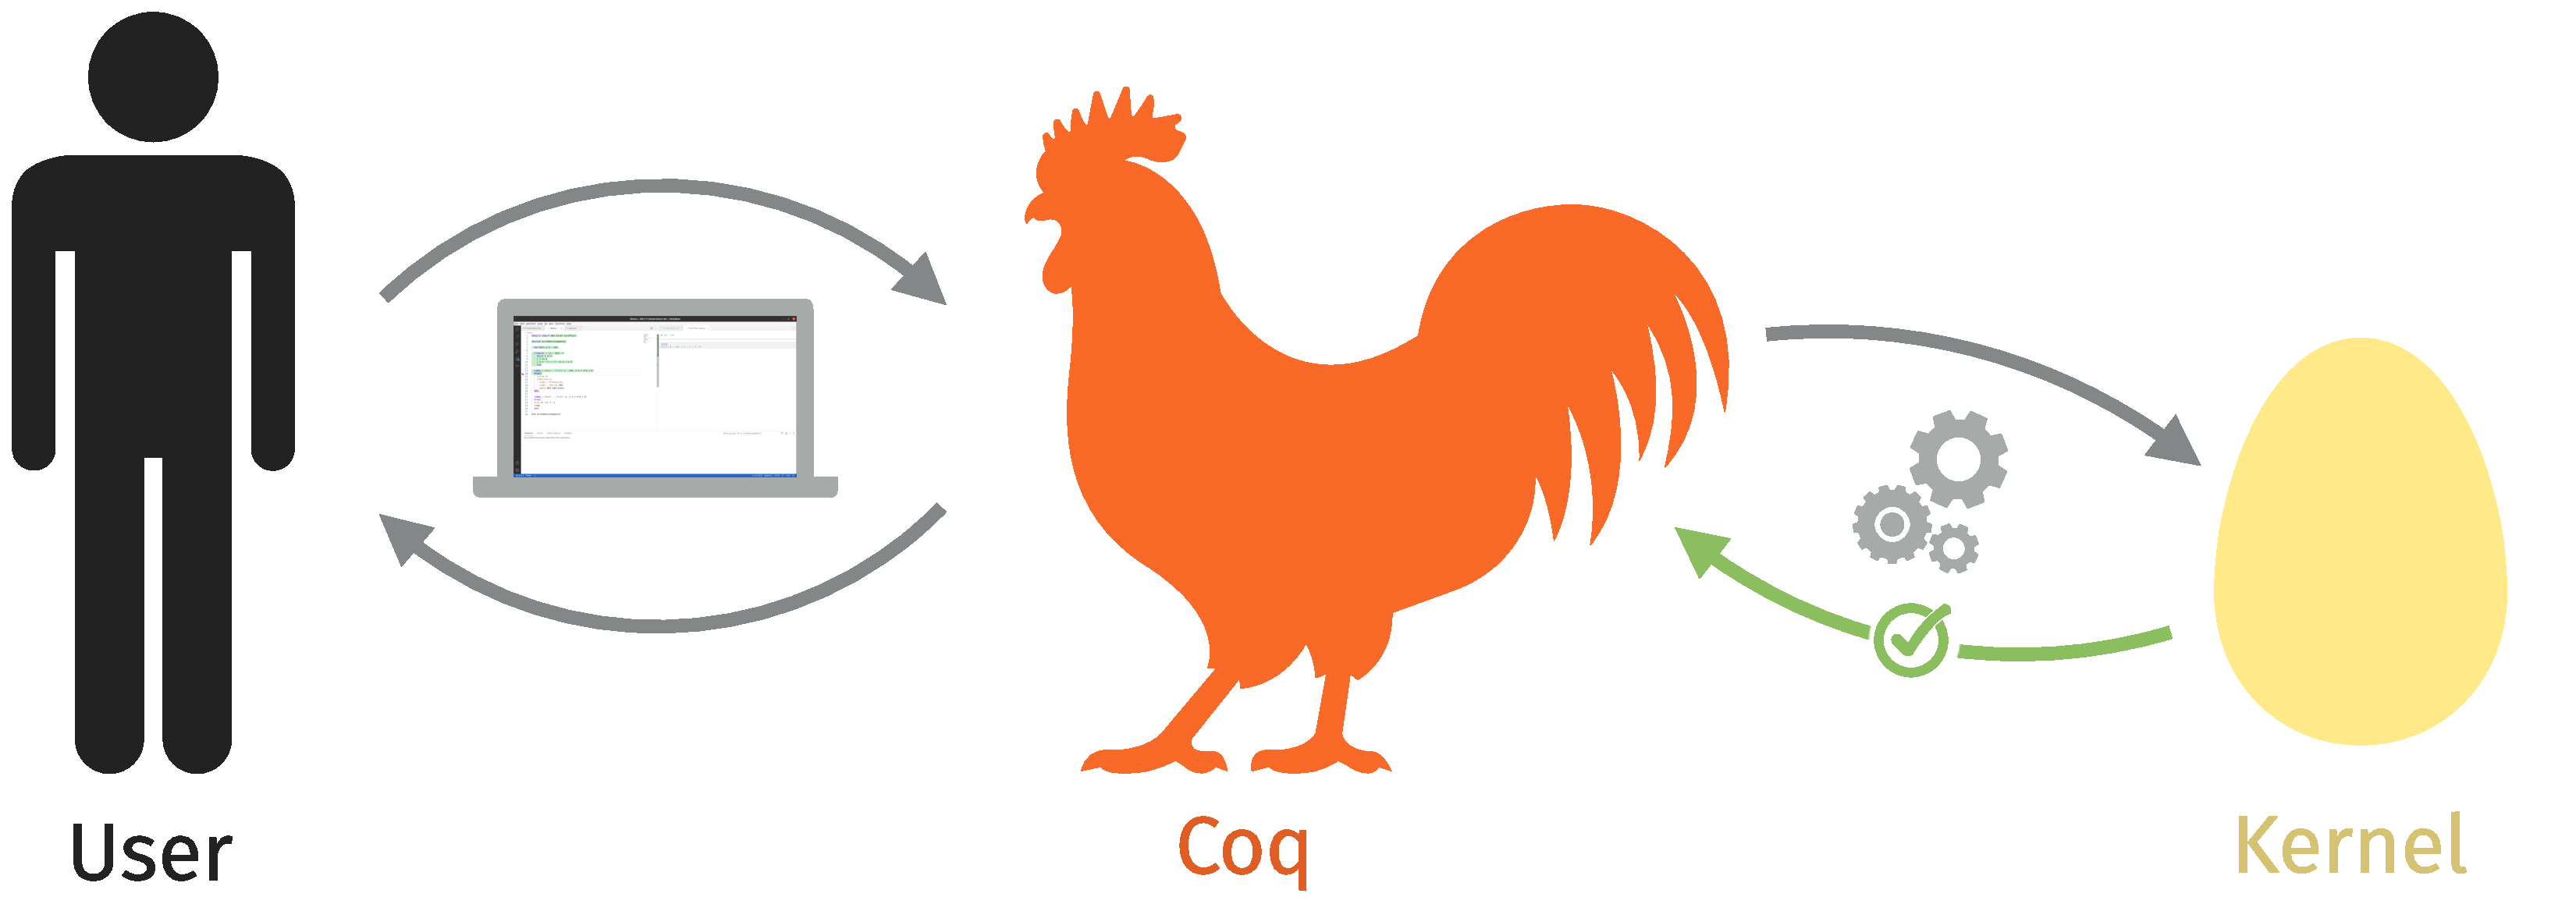
\includegraphics{./figures/coq-kernel-en.pdf}

  \caption{\kl{Coq}’s schematic architecture}
  \label{fig:coq-en}
\end{figure}

\kl{Coq} is based on the \kl{Curry-Howard correspondence}: proofs are seen as programs,
in a language called \intro{Gallina}, and their verification is done using an algorithm
close to those used for types in conventional languages. However, if, in the first versions
from the 80s, \kl{Coq} proof were mostly written directly in \kl{Gallina}, it is
no longer the case at all. The reason is that the major part of the tool in its
current versions aims at helping the user in generating a correct proof. It is a true
\kl[proof assistant]{proof \emph{assistant}}!
The way \kl{Coq} works is illustrated in \cref{fig:coq-en} : the user interactively exchanges
with \kl{Coq}, which uses this interaction to generate a proof term. This proof term is then
sent to a very specific part of the tool, called the \intro{kernel}.
This is the part implementing the type-checking algorithm, and thus responsible for ensuring
that the proof terms built interactively are correct.
The \kl{kernel} is thus the crucial part of \kl{Coq}, because it is the one – and only –
ultimately responsible for proof-checking.
This architecture, which clearly isolates the critical part of the system, is called
\intro{De Bruijn criterion} \sidecite{Barendregt2001}, in tribute to one of the pioneer
of proof assistants.

If the rest of the ecosystem has grown much more than the \kl{kernel} since the beginning,
the latter has also evolved, becoming gradually more complex.
And, as any other software development, it is not safe from bugs.%
\sidenote{The magnitude is that of one critical bug found every year, a list is maintained
at the following address: \url{https://github.com/coq/coq/blob/master/dev/doc/critical-bugs}.}
These are in general hard to exploit for a user, even more so without noticing.
But still, they exist, and since the \kl{kernel} tends to get more and more complex, they
are likely to continue appearing.

\subsection{\kl{MetaCoq}, a formalization in \kl{Coq}, for \kl{Coq}}[\kl{MetaCoq}]
\label{sec:intro-metacoq-fr}

If we wish to guarantee a trust level as high as possible in the \kl{kernel}, we must
resort to new ideas. This is what the \kl{MetaCoq} project is all about. The idea
is simple: use \kl{Coq} itself to certify the correctness of its \kl{kernel}.

More precisely, the first step is to describe formally the type system on which the \kl{kernel}
is based, and to show its theoretical properties.
This is already a difficult endeavour: in order to ease its use, \kl{Coq}’s type theory
incorporates a lot of complex features.

Once this meta-theory is established, the second step
% \sidenote{This is the one on which I mostly work, and on which we will come back in more
% length later on.}
consists in implementing a type-checking algorithm as close as possible to the one of the
\kl{kernel}, directly in \kl{Gallina}%
\sidenote{Indeed, thanks to the \kl{Curry-Howard correspondence}, \kl{Gallina} is not
only a proof language, but also a true programming language!}.
We show, while defining the algorithm, that it is indeed \reintro(bidir){sound}%
\sidenote{If the algorithm claims that a term is well-typed, then it is the case.}
and \reintro(bidir){complete}%
\sidenote{The algorithm answers positively on all well-typed programs.}.
Together, these two properties correspond to the \intro(bidir){correctness} of
the program.

Finally, in a third step, we extract out of this certified \kl{Gallina} program another
more efficient program, by erasing the content related to the proof of correctness, in order
to keep only the algorithmically relevant one.
This extraction is a complex but crucial step if we wish to replace the current \kl{kernel}
while keeping a reasonable efficiency. Therefore, we also prove that said extraction
is correct,%
\sidenote{Meaning that it preserves the semantics of programs.}
once again by programming it in \kl{Gallina}.

\subsection{Checking, inference and bidirectional typing}[Bidirectional typing]

While proving the correctness of the type-checker is relatively easy once the
meta-theoretical properties of the type system have been established, completeness is harder.
In order to prove it, it is very useful to go through an intermediate specification,
which is more structured than the theoretical one.
In particular, it is important to separate two close but distinct questions:
on the one side, type-checking, where we \emph{check} that a term indeed has a
given type;
on the other side, inference, where we try and \emph{find} a type for a term, if such a
type exists.
The typing algorithm of \kl{Coq}'s \kl{kernel} is \intro{bidirectional}, meaning that it
alternates constantly between these two processes when it checks that a term is well-typed.
Describing this bidirectional structure independently of the algorithm allows for a
clear separation between, on the one side, its equivalence with the original specification,
and, on the other, the part purely dedicated to implementation questions.

In the specific case of dependent types, even if present in type-checking algorithms since
the origin – see \eg \sidecite{Huet1989} –, bidirectional typing has been relatively little
studied. However, beyond its strong relation to algorithms, this approach also presents
theoretical advantages: its more constrained structure makes it easier
to obtain properties that are difficult to obtain in the standard context.

\subsection{Gradual types: some flexibility in a desperately static world}
  [Gradual types]
\label{sec:intro-graduel-en}

There are two main approaches to program type-checking. In the static approach,%
\sidenote{On which \kl{Coq} is based.}
types are verified prior to the execution, whereas, in the dynamic approach, the well-typedness
of operations is verified on the fly during that same execution.
The dynamic discipline is more flexible, as it checks exactly what is necessary
for the good execution of a program.
The strictness of static typing, conversely, allows for error detection earlier in the
development, and imposes invariants useful to optimize compilation or execution.

Instead of opting exclusively for one of the two approaches,
\reintro{gradual typing} \sidecite{Siek2015} aims at integrating
the static and dynamic disciplines in one and the
same language.
The main idea is to have a first pass of verification before the execution, as in static typing,
while leaving the possibility to defer parts of the verification to the execution, as in
dynamic typing.
This gives access to a whole spectrum of options, from a rigid completely static
discipline to a flexible dynamic one. It particularly allows for a fine-grained, local choice
of how each part of a program is type-checked.
One can thus evolve the discipline during software development, benefiting from
the flexibility of dynamic typing in early phases, and from the guarantees of static typing
later on.

As the case of \kl{MetaCoq} illustrates, \kl{Coq} can be used as a true programming language.
Even better: its type system can express very complex properties of programs, and thus
verify even before their execution that the code indeed enforces them.
Sadly, these reinforced constraints can turn against the user, by making the
early development phase more difficult. Indeed, nobody writes correct code on the first try,
and it would often be nice to temporarily lift the strong guarantees of typing to
facilitate experimentation. The idea then is to take inspiration from gradual typing,
in order to pave the way for a more flexible logical or software development. Once again, the
\kl{Curry-Howard correspondence} is at work, since we adapt concepts from the world of
programming languages to the logical one.

\section{And this Thesis?}
\label{sec:this-thesis}

My doctoral work itself is centred around bidirectional typing, under three main aspects,
corresponding to the three parts of this thesis.
They are preceded by \cref{chap:tech-intro}, which introduces the main technical notions
used in what follows.

\subsection{Theory of bidirectional typing}

The first part (\nameref{part:bidir}) proposes to – partially – fill the theoretical gap around
bidirectional typing for dependent types. More precisely, it contains a proof of equivalence
between the standard presentation of CIC in the literature, and a bidirectional one.
\Cref{chap:bidir-ccw} presents the main ideas in a relatively
simple setting, in order to ease the exposition. \Cref{chap:bidir-pcuic} shows how to extend
them to a more realistic setting, close to the type theory implemented in \kl{Coq}.
Finally, \cref{chap:bidir-conv} focuses on the particular status of conversion%
\sidenote{This crucial notion allows the integration into dependent type theory of
the notion of computation of programs.},
and the links between recent work on this subject and bidirectional typing.

\subsection{Bidirectional typing in \kl{MetaCoq}}

The second part of the thesis (\nameref{part:metacoq}) focuses on the \kl{MetaCoq} project,
and especially the formalization, in \kl{Coq}, of the ideas presented in the first part.
\Cref{chap:metacoq-general} gives a general overview of the project, while
\cref{chap:kernel-correctness} concentrates more specifically on the proof that the
\kl{kernel} implemented in \kl{MetaCoq} fulfils its specification.

\subsection{Gradual dependent types}

Finally, the third and last part (\nameref{part:gradual}) presents my work in the area
of \kl{gradual types}. Since dependent types already form complex systems, their adaptation
to the gradual approach is particularly delicate. A summary of the possibilities and issues is
presented in \cref{chap:gradual-dependent}. An interesting point of emphasis is that the
usual presentation of dependent types turns out to be unsuited, as it is too flexible.
The additional structure provided by bidirectional typing is key to solve this issue. It is also
relevant to present the type-directed elaboration of terms from a source language
to a target one, an important characteristic shared by all \kl[gradual types]{gradual languages}.
The use of a bidirectional elaboration, and the properties it allows us to obtain, are described
in \cref{chap:bidir-gradual-elab}. Finally, \cref{chap:beyond-gcic} describes follow-up work
complementing that of \cref{chap:bidir-gradual-elab}, but which is not directly linked to
bidirectional typing.

\subsection{Technical contributions}

My doctoral work started with the study of \kl(typ){gradual}
\kl(typ){dependent} types.
I contributed, together with Kenji Maillard, Nicolas Tabareau and Éric Tanter, to
\sidetextcite{LennonBertrand2022}, where we study a gradual extension to the
Calculus of Inductive Constructions. My main technical contribution corresponds
to \cref{chap:bidir-gradual-elab}. The precise literature review and the impossibility
theorem of \cref{chap:gradual-dependent} it leads to also comes from this
publication.
The second technical part of \textcite{LennonBertrand2022}, in which I participated but
whose main author is Kenji Maillard, as well as a second article,%
\sidenote{\textcite{Maillard2022}, currently under review.}%
\margincite{Maillard2022}
together with the same authors and again Kenji Maillard as main investigator,
correspond to \cref{chap:beyond-gcic}.

This work having shown the relevance of a bidirectional dependent type system and the relative
scarceness of results on the subject, I focused more closely on it, both on
paper and by means of a formalization based on \kl{MetaCoq}. This led to a second publication
\sidecite{LennonBertrand2021}, and corresponds to \cref{chap:bidir-ccw,chap:bidir-pcuic}
for the theoretical part, and \cref{sec:kernel-bidir} for the formalized proof
of equivalence between bidirectional and undirected typing.
The completeness bug in the kernel of \kl{Coq} found during this formalisation, together with
the impact of this discovery on the implementation of \kl{Coq} is presented in
\sidetextcite{Sozeau2022}.

I then turned to the closer integration of this formalization into \kl{MetaCoq}, and its use
in order to prove completeness of the \kl{kernel} it implements.%
\sidenote{A definition of a type-checking algorithm proven sound but not complete by
Simon Boulier was already present, although I had to alter it during the completeness
proof.}
This is described in \cref{sec:kernel-typing}.
I also contributed more generally to the project on various more minor points.
This part of my thesis work has not been published yet, but the other contributors to
\kl{MetaCoq} and I are currently working on it.

Finally, \cref{chap:bidir-conv} corresponds to a project I initiated in order to extend
\kl{MetaCoq} to integrate extensionality η rules to conversion,
but which did not reach the stage of publication yet. Yet, I presented the difficulties
that led me to it in \sidetextcite{LennonBertrand2022a}.

\end{comment}
